% This is samplepaper.tex, a sample chapter demonstrating the
% LLNCS macro package for Springer Computer Science proceedings;
% Version 2.20 of 2017/10/04
%
\documentclass[runningheads]{llncs}
%

\usepackage{caption} 
\captionsetup[table]{skip=10pt}

\usepackage{graphicx}
\usepackage{multirow}
\usepackage[section]{placeins}
% Used for displaying a sample figure. If possible, figure files should
% be included in EPS format.
%
% If you use the hyperref package, please uncomment the following line
% to display URLs in blue roman font according to Springer's eBook style:
% \renewcommand\UrlFont{\color{blue}\rmfamily}
	
\begin{document}
%
\title{Difficulty classification of mountainbike downhill trails utilizing deep neural networks}
%
%\titlerunning{Abbreviated paper title}
% If the paper title is too long for the running head, you can set
% an abbreviated paper title here
%
\author{Stefan Langer\inst{1}}
%
\authorrunning{Stefan Langer et al.}
% First names are abbreviated in the running head.
% If there are more than two authors, 'et al.' is used.
%
\institute{LMU Munich
\email{stefan.langer@ifu.lmu.de\inst{1}}\\
\url{http://www.mobile.ifi.lmu.de} }
%
\maketitle              % typeset the header of the contributionY>
%
\begin{abstract}
The difficulty of mountainbike downhill trails is a subjective perception. 
However, trails are grouped into difficulty grades with scales like the "Singletrail-Skala" (S0-S5) or  colored scales (blue, red, black, ...).
The latter is mostly being used in dedicated mountainbike parks and in North America.
We propose an end-to-end deep learning approach to classify trails into the three difficulties easy, medium, and hard.
With mbientlab Meta Motion r0.2 sensor units, we record accelerometer- and gyroscope data of rides down multiple trails.
We train a 2D convolutional neural network with a stacked and concatenated representation of the aforementioned data as its input.
We run experiments with three different sample- and three different kernel sizes.
We achieve a sparse categorical accuracy of 82\% on our test data set.
As to our knowledge this is the first work utilizing deep neural networks for mountainbike sports analytics and the first work targeting computational difficulty classification of mountainbike downhill trails.


\keywords{Sports analytics  \and Deep neural networks \and Accelerometer \and Gyroscope \and Convolutional neural networks.}
\end{abstract}
%
%
%
\section{Introduction}
Mountainbiking is a popular sport amongst outdoor enthusiasts, comprising many different styles.
There are styles like cross country riding, characterized by long endurance rides, styles like downhill riding, characterized by short, intense rides down trails, and more.
Mountainbiking, as it is known today, originated in the US in the 1970s and has passed through various levels of popularity since~\cite{gaulrapp2001injuries}.
Official, competitive riding started in the 1980s with the foundation of the Union Cycliste Internationale (UCI), followed by the first World Championship in 1990 ~\cite{impellizzeri2007physiology}. 
In this work, we focus on the difficulty classification of mountainbike downhill trails and do not take into account uphill or flat sections of trails.
There are multiple approaches in trail difficulty classification, wherebys a color-inspired grading seems to be common ~\cite{imbarating,britishcyclinggrades,schymik2008singletrail}.
The International Mountain Bicycling Association (IMBA) proposes a trail difficulty rating system comprising five grades ranging from a green circle (easiest) to a double black diamond (extremely difficult) ~\cite{imbarating}. 
In addition, the IMBA Canada offers a guideline on how to apply those gradings to mountainbike trails ~\cite{imbaguidelines}.
British Cycling also propose a colored difficulty scale comprising four basic grades, ranging from green (easy) to black (severe) with an additional orange for bike park trails ~\cite{britishcyclinggrades}.
Inspired by  rock climbing difficulty grading as well as ski resort gradings, Carsten Schymik et al. created the "Singletrail-Skala", containing three main difficulty classes (blue, red, black) and a more fine granular six grades ranging from S0 to S5 ~\cite{schymik2008singletrail}. 
Trails on openstreetmap.org are rated in respect to the IMBA grading as well as the Singletrail-Skala, wheareas the latter also describes tracks which are not made for mountainbiking ~\cite{osmsingletrails}. 
Because there are multiple trail gradings and due to a rather subjective estimation of the difficulties it is not an easy task to find the right rating of a downhill trail.
With this work we want to make moutainbike track difficulty assessment less subjective and more measurable.
In order to do so, we collect acceleration-, as well as gyroscope-data from multiple sensor units that are connected to the mountainbike frame as well as the rider.
Because we collect data not only in dedicated bikeparks, but also on open trails (hiking paths among others), we decide to use the three main difficulties given by the Singletrail-Skala as the set of labels.
Table~\ref{table:coloredgrading} gives an overview of the three grades blue, red and black.
Schymik et. al define the difficulties as follows ~\cite{osmsingletrails}:
Blue describes easy trails, comprising the grades S0 and S1.
Red describes medium trails and is equal to the grade S2.
Black describes all difficulties above and can be considered hard.
Openstreetmap.org provide difficulty classifications for all trails on which this dataset is collected ~\cite{osmsingletrails}.
We then train a 2D convolutional neural network with a stacked and concatenated representation of the aforementioned data as its input.
Thereby we can grade sections of downhill trails regarding their difficulty.


\subsection{Mountainbike analytics and sensor data analysis}
For training purposes, mountainbikes of professional athletes get set up with telemtry technology, such as BYB Telemetry's sensors ~\cite{bybtelemetry}.
Their sensors are connected to the suspension fork as well as the suspension shock and measure the movement of each.
Stendec Data extends those capabilities and adds sensors for measuring brake pressure and acceleration in order to capture braking points, wheel movements, and more ~\cite{stendecracing}.
However, the two systems mentioned above are expensive and hard to get.
We therefore use mbientlab Meta Motion sensor units to capture acceleration and gyroscope data.
To our knowledge there is no scientific work regarding the difficulty classification of mountainbike trails using accelerometers or gyroscopes yet.
However, there has been a great amount of work done in the field of activity recognition with acceleration data ~\cite{ravi2005activity,bao2004activity,kwapisz2011activity,lara2012survey,yang2015deep,zeng2014convolutional,ronao2016human}.
Many of those approaches make use of classical machine learning methods ~\cite{ravi2005activity,bao2004activity,kwapisz2011activity,lara2012survey,preece2008comparison}.
S. J. Preece et al. compare feature extraction methods for activity recognition in accelerometer data ~\cite{preece2008comparison}.
Ling Bao et al. classify activities using custom algorithms and five  biaxial acceleration sensors worn simultaneously on different parts of the body ~\cite{bao2004activity}.
Furthermore, there has been a noticeable shift towards deep learning approaches in recent years ~\cite{yang2015deep,zeng2014convolutional,ronao2016human}.
Fernando Moya Rueda et al. use multiple convolutional neural networks which they concatenate in a later stage with fully connected layers ~\cite{moya2018convolutional}.
Zeng et al. utilize a 1D convolutional neural network, treating each axis of the accelerometer as one channel of the initial layer ~\cite{zeng2014convolutional}.
In a survey by Jindong Wang et al., the authors give an overview of state-of-the art deep learning methods in activity recognition and claim that deep learning has been widely adopted for sensor-based activity recognition tasks~\cite{wang2019deep}.


\section{The dataset}

\subsection{Collecting and labeling data}

\begin{figure}
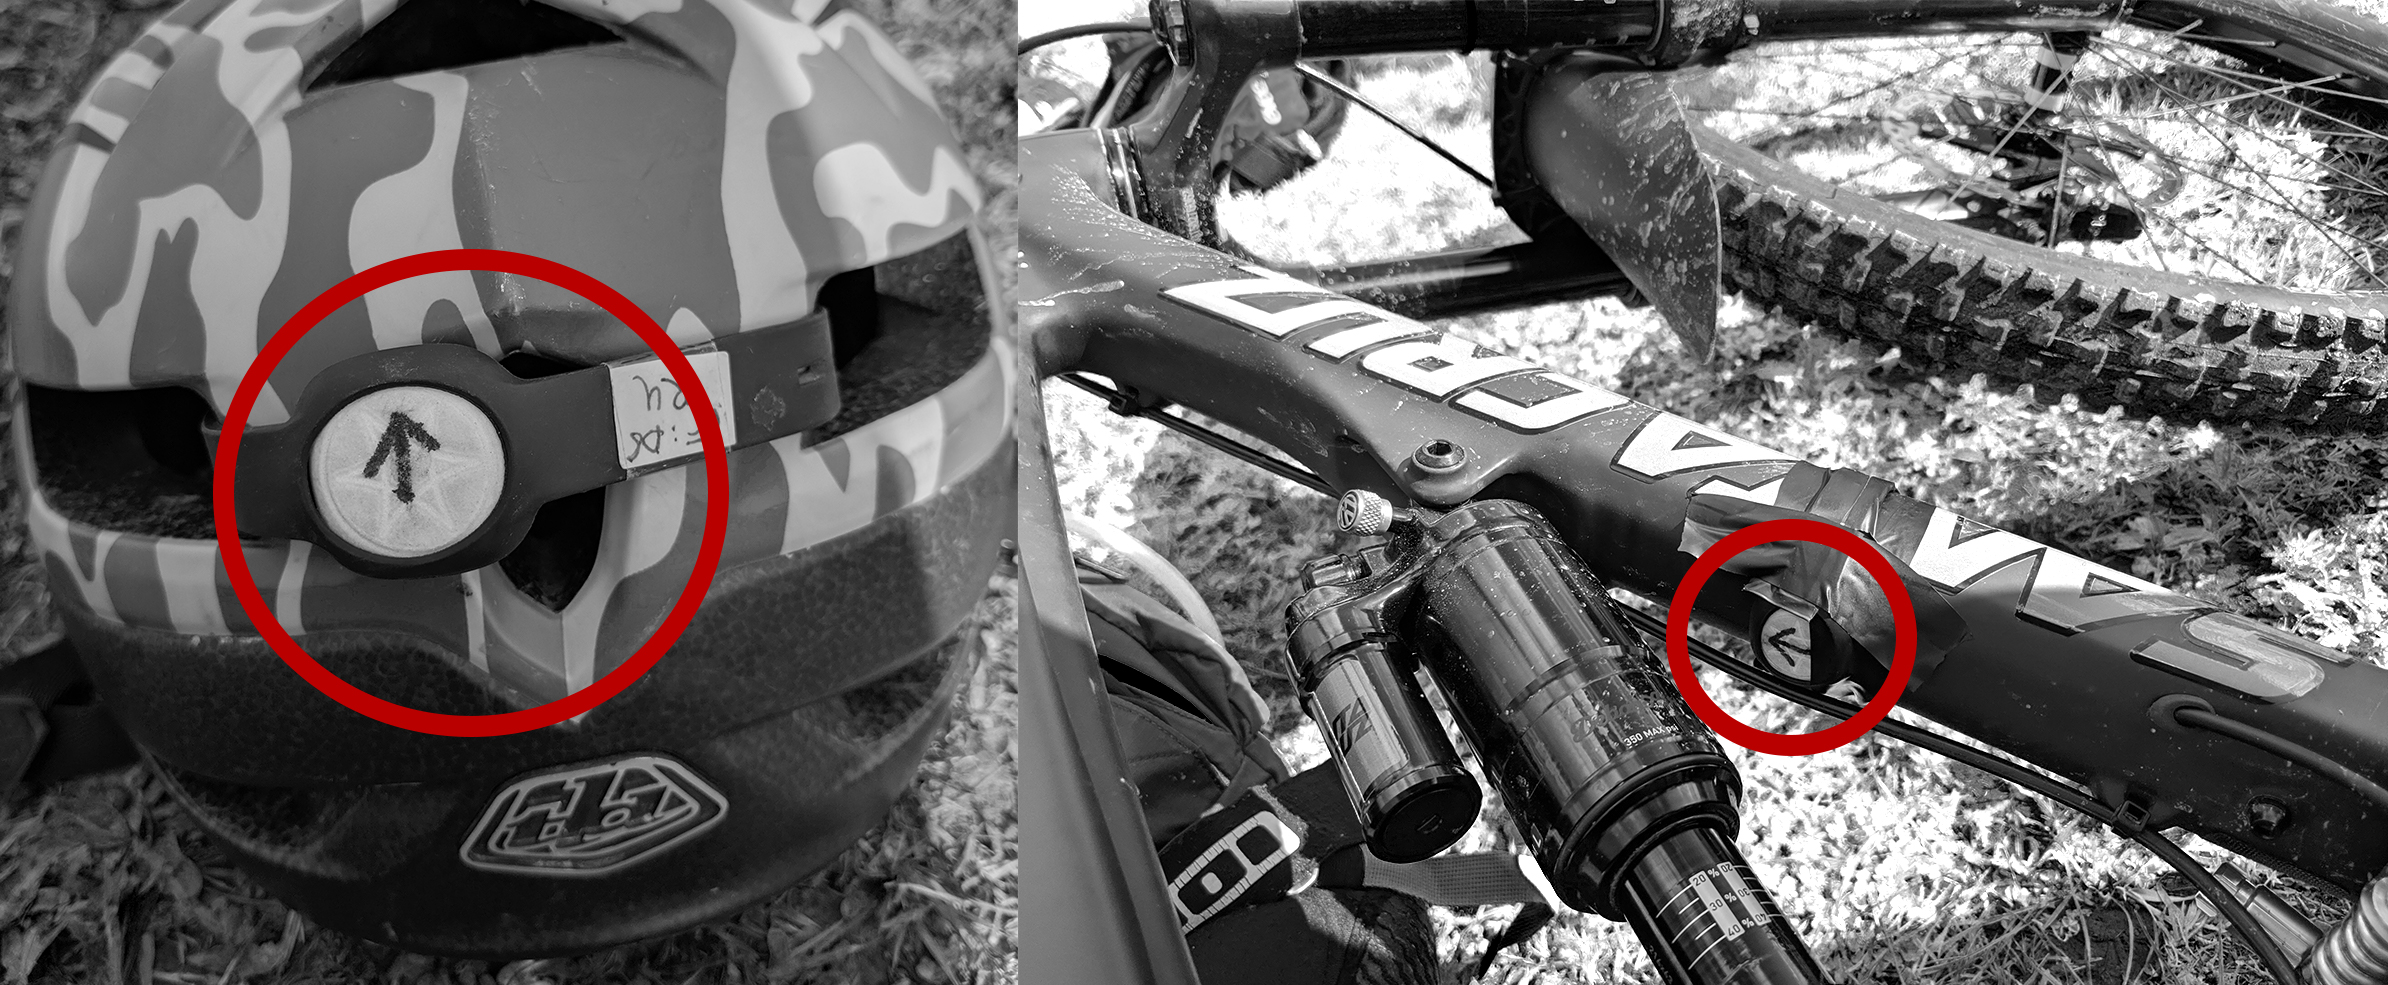
\includegraphics[width=\textwidth]{mountingpoints.jpg}
\caption{Mounting point on the helmet (left), mounting point on the downtube of the frame (right)}
\label{fig1}	
\end{figure}

Instead of working with dedicated mountainbike telemetry systems, we use mbientlab Meta Motion r0.2 sensor units to record data ~\cite{mbientlab}.
Those units contain multiple sensors including an accelerometer as well as a gyroscope, which we both use for collecting data.
Mbientlab sensors offer a Bluetooth Low Energy interface to which an Android or iOS application can be connected.
The app allows to group two or more sensor units in order to record from both simultaneously.
Riders are equipped with two units that are connected to one smartphone.
Fig.~\ref{fig1} visualizes the mounting points of the mbientlab sensor units.
One unit is connected to the downtube of the mountainbike, the other one to the back of the riders helmet.
For each recording, the sensors are facing the same direction to keep the axes layout consistent.
The accelerometer creates datapoints in three axes (x, y, z) in the unit g (equals $9.80665 m/s^2$) with a frequency of 12.5Hz.
The gyroscope creates datapoints in three axes (x, y, z) in the unit deg/s with a frequency of 25.00Hz.
We synchronize the starting points of the recordings and linearly interpolate missing datapoints to reach a constant frequency of 25.00Hz for all sensors.

\begin{table}[]
\centering
\resizebox{\textwidth}{!}{%
\begin{tabular}{|l|l|l|l|}
\hline
Colored grading & Fine grading & Label & Description                                                                                                                                                    \\ \hline
blue            & S0, S1       & 0     & \begin{tabular}[c]{@{}l@{}}Easy. \\ Mostly solid and non-slip surface. \\ Slight to moderate gradient. \\ No switchbacks. \\ Basic skills of need.\end{tabular}         \\ \hline
red             & S2           & 1     & \begin{tabular}[c]{@{}l@{}}Medium. \\ Loose surface, bigger roots and stones.\\ Moderate steps and drops.\\ Moderate switchbacks.\\ Advanced skills of need.\end{tabular} \\ \hline
black           & S3+          & 2     & \begin{tabular}[c]{@{}l@{}}Hard. \\ Loose surface, slippery, big roots and stones.\\ High drops.\\ Tight switchbacks.\\ Very good skills of need\end{tabular}           \\ \hline
                &              & 3     & \begin{tabular}[c]{@{}l@{}}Not riding the bike.\\ Breaks inbetween the ride or when carrying \\ the bike across obstacles like trees.\end{tabular}                                         \\ \hline
\end{tabular}%
}
\caption{Mapping of the Singletrail-Skala grades to the labels used in our data set. Labels 0-2 represent the  difficulties, label 3 represents non-riding segments.}
\label{table:coloredgrading}
\end{table}

Labeling of the data happens after the actual data collection process.
We record every downhill ride with an action camera (mounted to the rider's chest), synchronize the video with the data recordings, and manually label subsections of the trail.
For the majority of subsections on open trails, we use the difficulty grading provided by openstreetmap.org.
For dedicated trails in mountainbike parks we use the difficulty classification given by the provider.
For subsections that the Singletral Skala would consider to not represent this difficulty, we up- or downgrade the difficulty label.
Downgrading mostly occurs for fireroads or other very easy sections, upgrading for particularly steep or tight sections.
For breaks inbetween the downhill ride or when carrying the bike across obstacles like trees, we introduce the additional label 4 (see table~\ref{table:coloredgrading}).

\subsection{Input data representation}

\begin{figure}
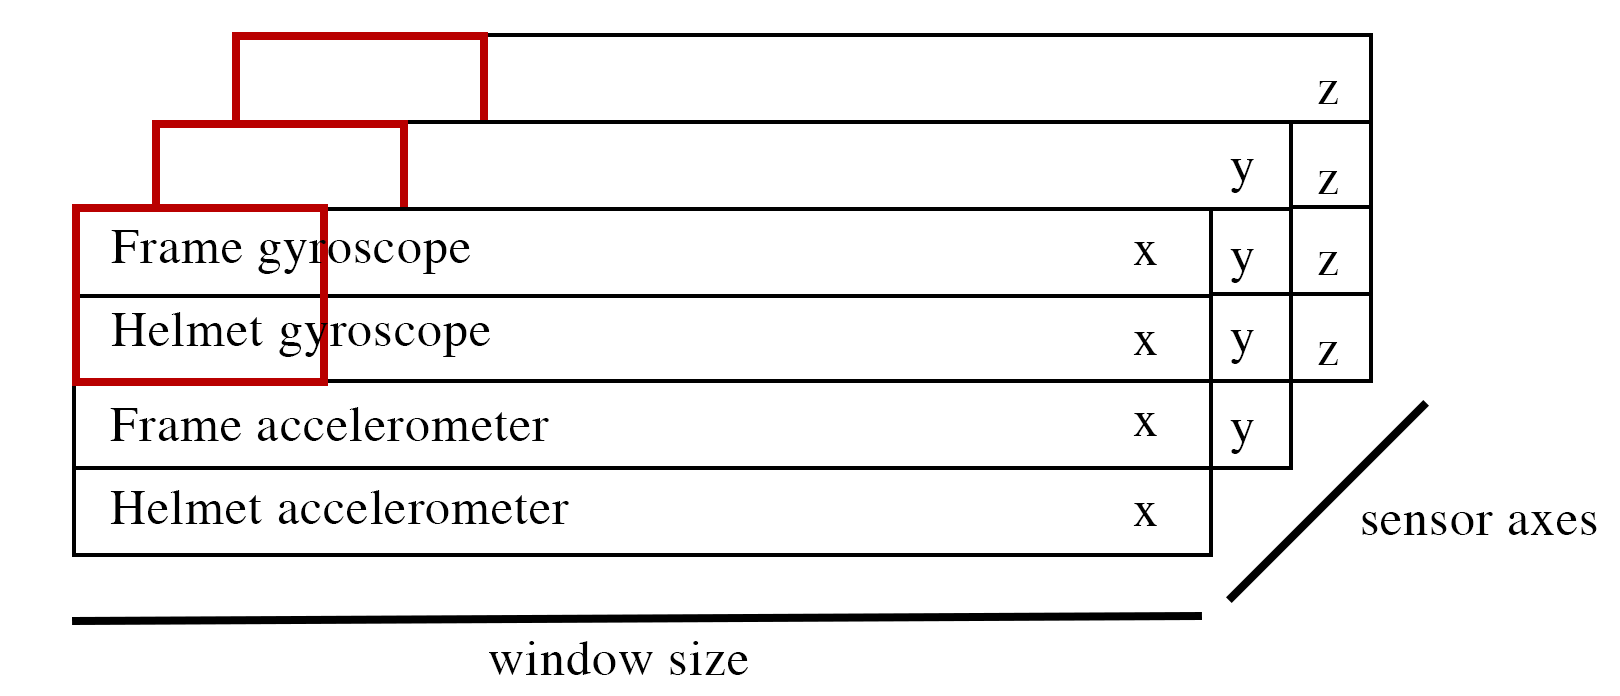
\includegraphics[width=\textwidth]{input_shape.png}
\caption{Input shape of one sample comprising 4 sensors with 3 dimensions (axes) each}
\label{fig2}	
\end{figure}

For each rider, we collect data with two sensor units.
Every unit provides data for the accelerometer and the gyroscpope sensors.
Each sensor provides datapoints for three axes (x, y, z) with an additional timestamp value.
Zeng et al. interpret each axis of a sensor as a filter of the input to a 1D convolutional layer ~\cite{zeng2014convolutional}.
We keep the same procedure but additionally stack each of the four sensors (two accelerometers, two gyroscopes) vertically to create an image-like representation.
Fig.~\ref{fig2} visualizes the shape of our input data.
Height and width are represented by sensors and datapoints of a sample.
RGB-like channels are represented by the three axes x, y, and z.
The square in the top left corner visualizes the kernel sliding across the input data.
We split each recording into smaller samples utilizing a sliding window with an overlap of 75\%.
This allows us to create many examples from few data recordings.
In our experiments we test three different window sizes, namely 1000ms, 5000ms, and 10000ms, resulting in 25, 125 and 250 data points per sample.


\section{Classification through a 2D convolutional neural network}

\begin{figure}
\centering 
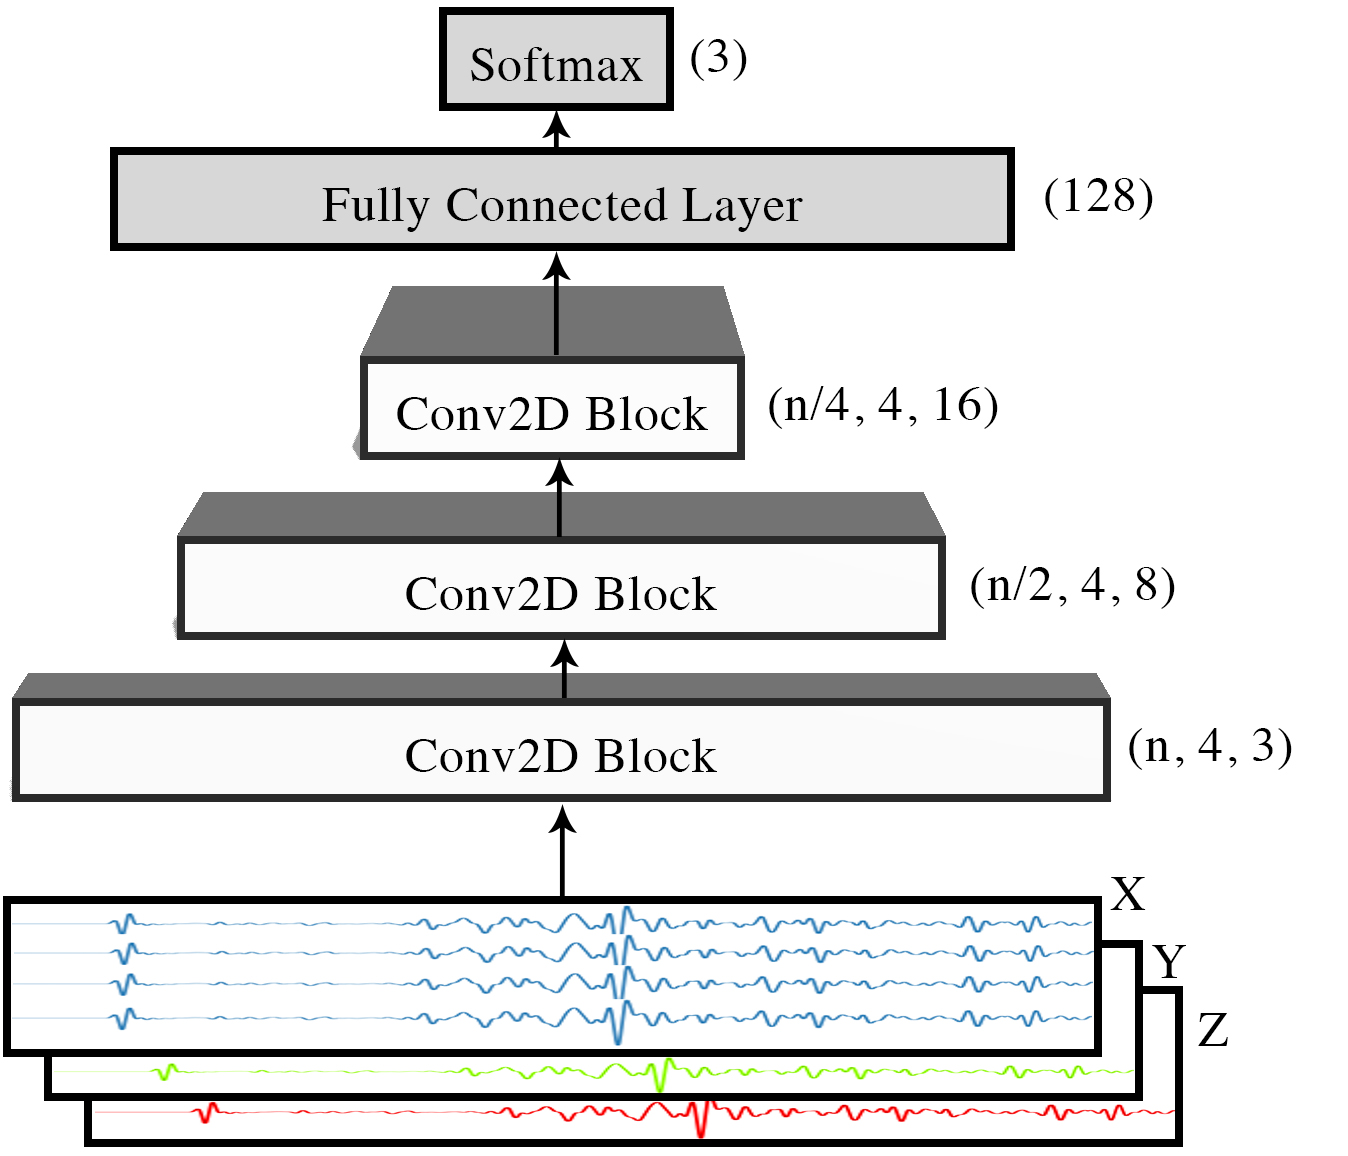
\includegraphics[width=0.70\textwidth]{network.jpg}
\caption{Convolutional Neural Network for trail difficulty classification on stacked accelerometer and gyroscope data. 
The input data is of shape (n, 4, 3), with n being the amount of data points per sample. 
After the input layer three convolutional blocks (consisting of Conv2D, Batch Normalization, Activation, Max Pooling and Dropout layers) and two fully connected layers follow.
The last layer results in a softmax activation.}
\label{fig3}	
\end{figure}

Fig.~\ref{fig3} visualizes our convolutional neural network.
The input to the first block is of shape (n, 4, 3), with n being the amount of data points per sample. One sample comprises data of 4 sensors (vertically stacked) with each three axes (filters) and a sample size of m data points.
We chain three Convolutional blocks followed by two Dense Layers.
Each Convolutional Block consists of one Conv2D, a Batch Normalization, a Relu Activation, a Max Pool and a Dropout Layer.
The convolutional layers use a kernel of shape (m, 2) and a stride of (1, 1), with m being the length of the kernel.
Multiple values for n and m are tested in the experiments.
All convolutional layers use the padding 'same' and L2 regularization.
After Batch Normalization we activate the units with a standard relu activation.
Max Pool layers use a pool size of (2, 1), which reduces the shape by approximately half in length.
The dropout rate of each Dropout Layer is 0.3.
The Conv2D Layers of the second and third Convolutional Block have 8 and 16 layers respectively.
After the Convolutional Blocks, we add two Dense Layers. 
The first layer has 128 units and a relu activation.
The second and final layer has four Softmax activated units, which represent the predicted label.
The network uses the Adam optimizer with a learning rate of 1e-3 and a Sparse Categorical Crossentropy as its loss function.

\FloatBarrier
\subsection{Experiments}

Because there are no established neural network configurations for trail difficulty classification, we test combinations of multiple window- as well as kernel sizes.
We execute 90 complete runs in total, composed of ten times per window-size/kernel-size combination.
We test the three window sizes 1000ms, 5000ms, 10000ms and the three kernel sizes (5,2), (10,2), (20, 2).
In order to reduce overfitting we add an Early Stopping callback to the network, which stops the training process when there is no improvement for 48 epochs.
We run a batch size of 32 and a steady learning rate of 1e-3.
In table~\ref{table:configurations} we show the resulting sparse categorical accuracy, the amount of epochs before training was stopped and the amount of samples in the train and test set.
For every experiment, we use a sliding window with an overlap of 75\%.
To not have many highly similar examples in one batch, we shuffle the data before training.
Every configuration uses the Adam optimizer, a dropout rate of 0.3, Relu activation for the hidden layers and a softmax activation for the output layer.
With a long window size of 10000ms, we achieve the worst results with all kernel sizes.
Overfitting starts early, resulting in a rapidly decreasing sparse categorical accuracy.
This could be attributed to the low amount of samples (TODO: Amount of samples) resulting of a long window size, as well as overlapping labels within a sample.
We observe better results for a window size of 5000ms and the largest kernel with shape (20,2).
However, the validation accuracy seems to decrease quickly and not increase before Early Stopping cancels the learning process.
For all kernel sizes, a window size of 1000ms offers highly improved results.
The best result is achieved for a kernel size of (20,2) (see table~\ref{table:configurations}).
Fig.~\ref{fig4} shows the curves of the Sparse Categorical Accuracy on the train as well on the test dataset across TODO epochs. %TODO
Both values increase early on and level out with no major overfitting visible in the plot.
This leads to the conclusion, that a subsection of 1000ms is enough to represent downhill difficulty.
Using a bigger kernel, and therefore longer sequential dependencies, leads to a better performance as well.
Fig.~\ref{fig3} shows the confusion matrix of the best resulting configuration, namely 1000ms and a kernel of (20,2).
It shows a good result with only minor false positives in neighbored areas. An especially good accuracy in classifying "non riding" (label 3) can be seen.
However, the matrix also highlights the fact, that the label 2 (hard) is underrepresented.

\begin{table}[]
\centering
\begin{tabular}{ll|l|l|l|l|}
\cline{3-6}
                                                    &         & \multicolumn{3}{l|}{Kernel sizes} & Samples \\ \cline{3-6} 
                                                    &         & (5,2)     & (10,2)    & (20,2)    &         \\ \hline
\multicolumn{1}{|l|}{\multirow{3}{*}{Window sizes}} & 1000ms  & 0.5       & 0.5       & 0.5       & 1000    \\ \cline{2-6} 
\multicolumn{1}{|l|}{}                              & 5000ms  & 0.5       & 0.5       & 0.5       & 500     \\ \cline{2-6} 
\multicolumn{1}{|l|}{}                              & 10000ms & 0.5       & 0.5       & 0.5       & 100     \\ \hline
\end{tabular}
\caption{Sparse Categorical Accuracy of multiple kernel an window sizes. A window size of 5000ms with a kernel size of (10,2) creates the highest sparse categorical accuracy on the test dataset.}
\label{table:configurations}
\end{table}

\begin{figure}
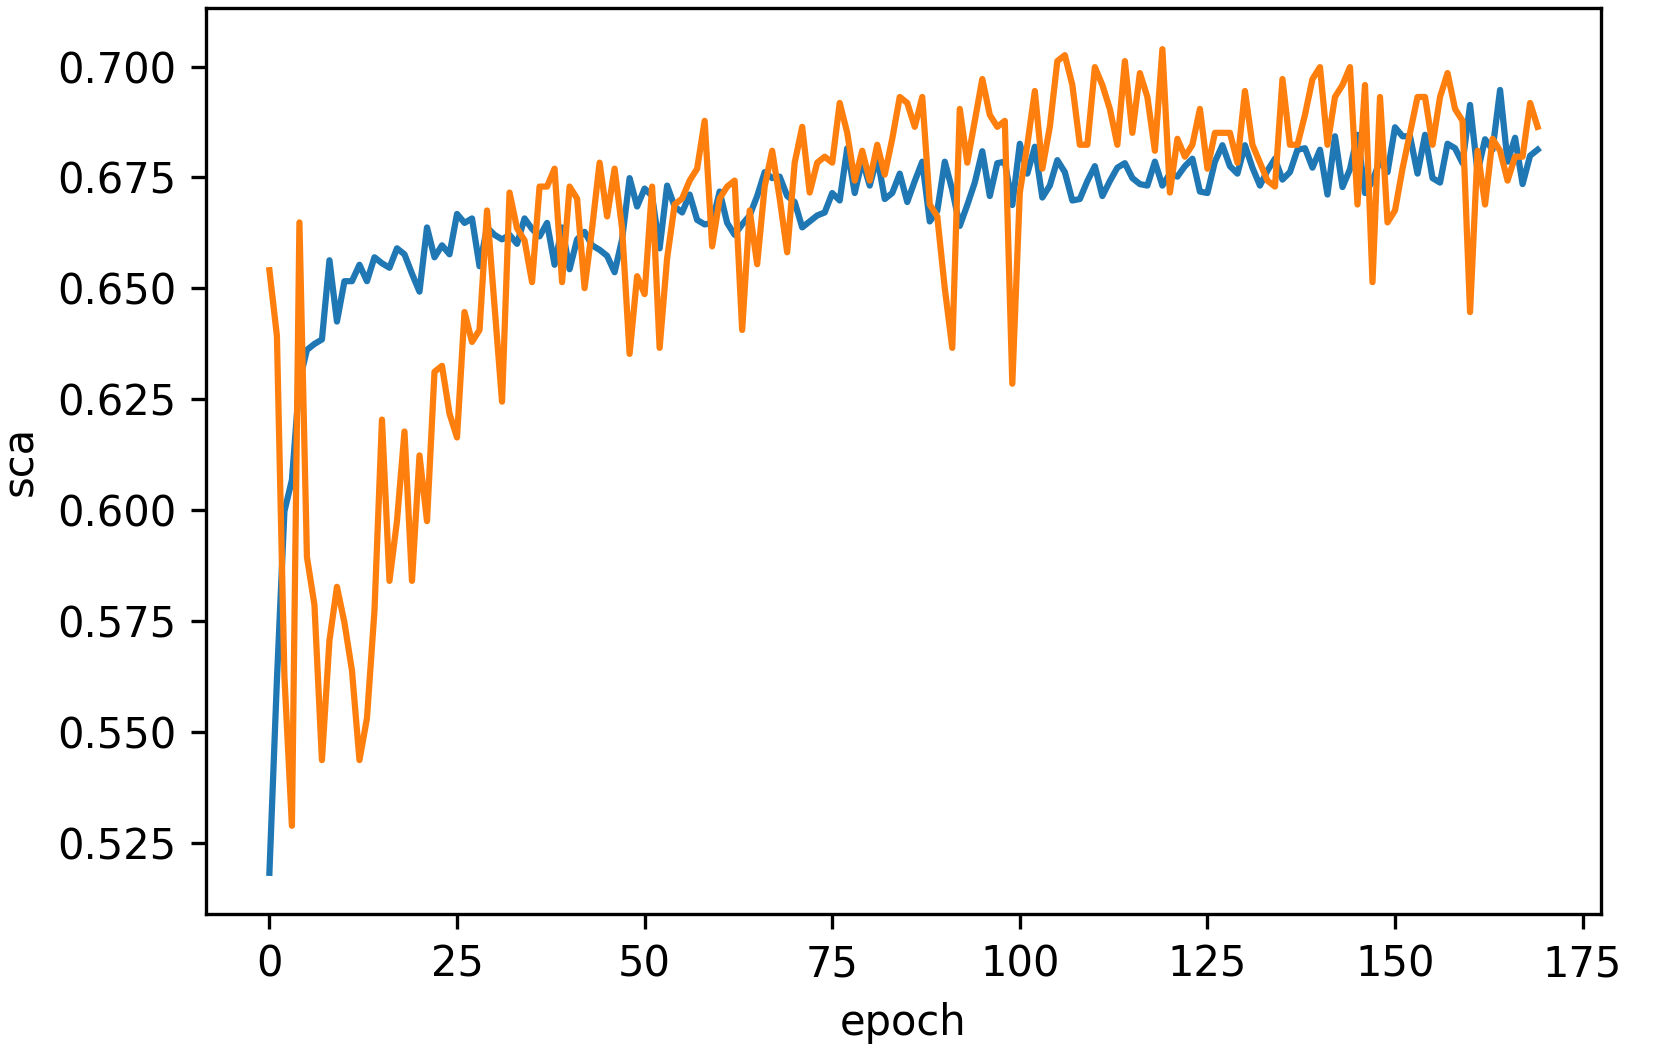
\includegraphics[width=\textwidth]{accuracy_plot.png}
\caption{Plot of the Sparse Categorical Accuracy (sca) on the train set (blue) as well as on the test set (orange). Both curves level out early on, not drifting apart, presuming a low amount of overfitting.}
\label{fig4}	
\end{figure} 



\begin{figure}
\centering 
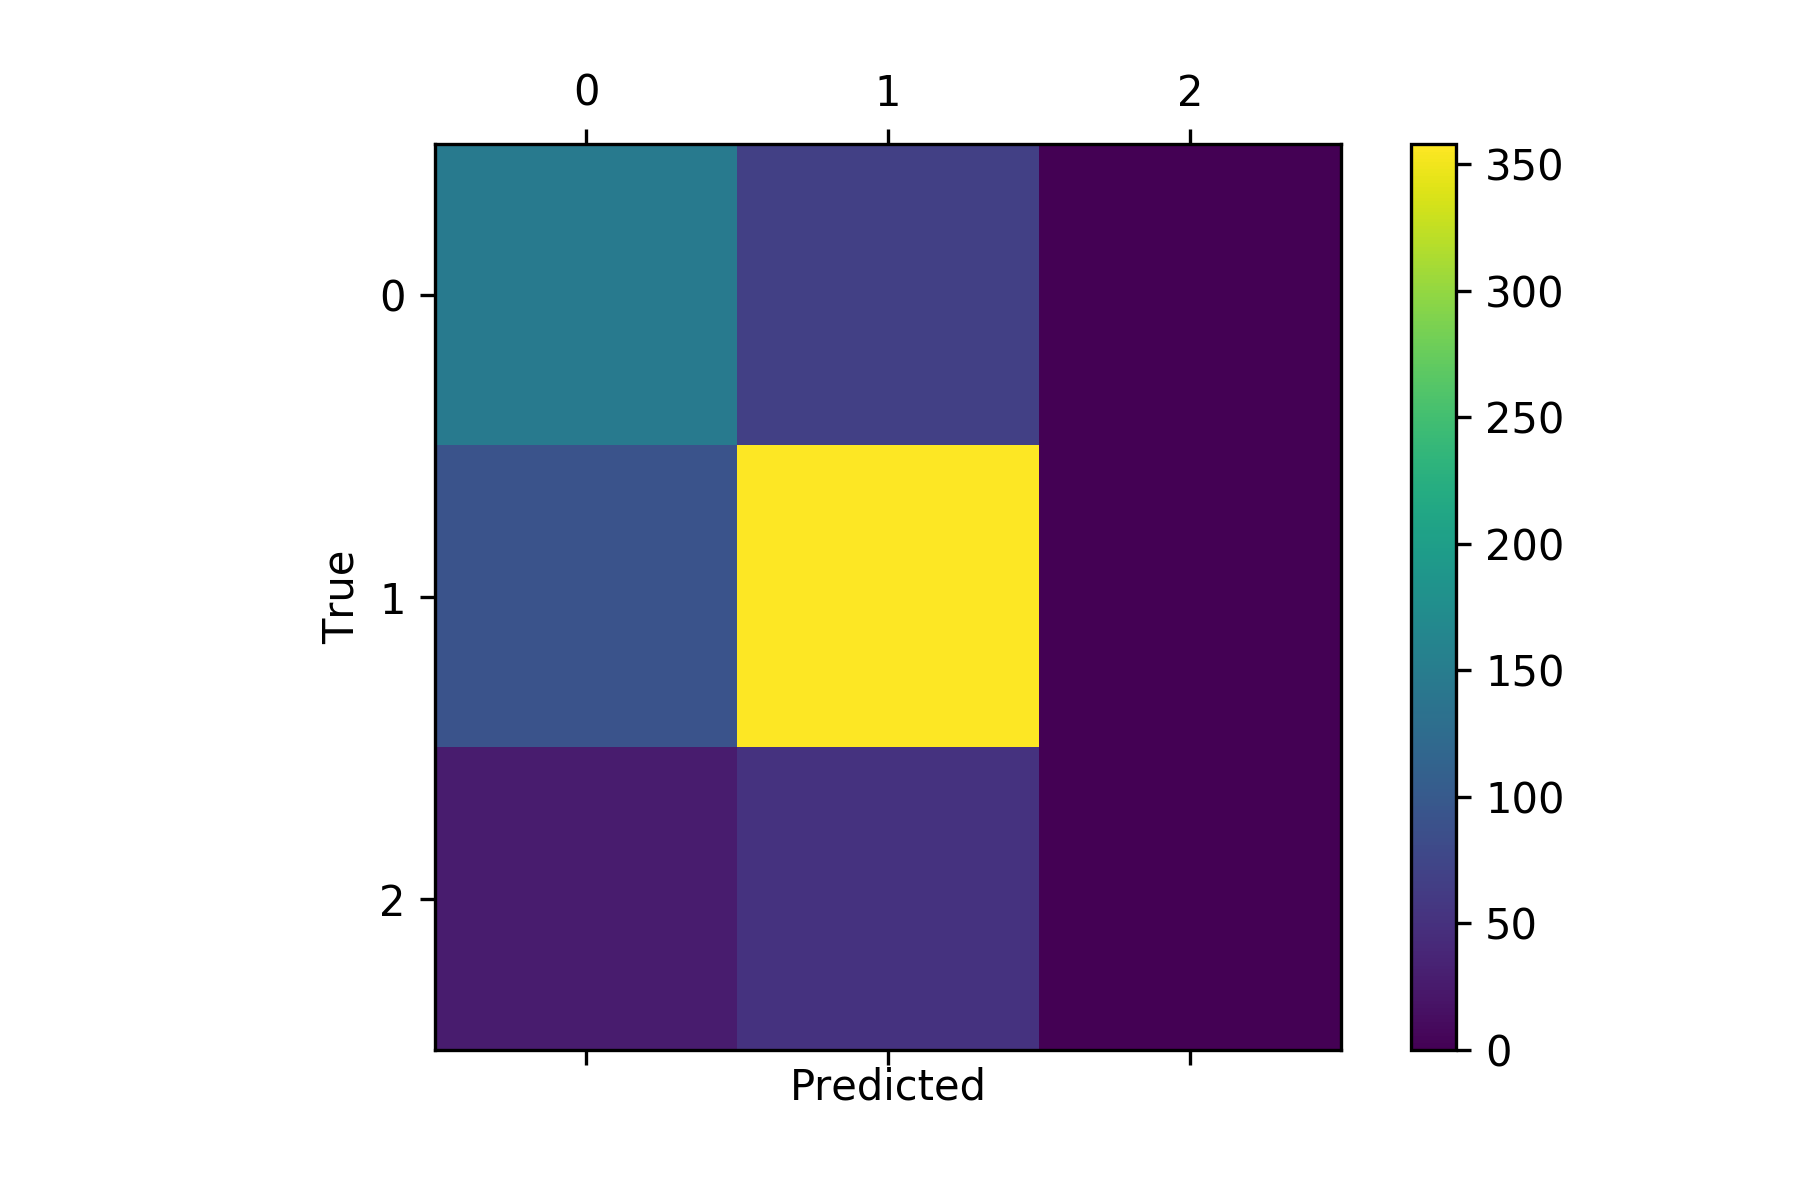
\includegraphics[width=0.70\textwidth]{confusionmatrix.png}
\caption{The confusion matrix on the test dataset shows a good result with only minor false positives in neighbored areas. A underrepresentation of the label 2 (hard) is noticeable.}
\label{fig3}	
\end{figure}




% TODO:  Parameter values have to be changed in the Net description above as well

%\subsection{Unsupervised clustering with PCA and K-means}
%TODO
%In addition to the aforementioned, well working result, we compared two clustering methods
%The first one being a very common architecture of PCA and K-Means [x, y, z, zz].
%We use the same amount of clusters
%For each resulting cluster, we let a majority vote decide it's label, which resulted in label "1" in the majority of times.
%Additionally, we combined a PCA with DBSCAN and let the algorithm decide on how many clusters on its own
%DBSCAN results in 2 clusters.
%We let a majority vote decide it's label, which resulted in label "1" (medium) and label "3" (not riding)
%This can be interpreted as "riding" and "not riding", so is therefore not suitable for difficulty classification in this setting.
%However, we are aware of the tuneability of the aforementioned clustering algorithms.
%This, however might need hand-crafted feature engineering, dimension reduction and specific domain knowledge.
%Our approach shows eliminates those steps and reaches a good accuracy.
%Cite SkLearn!


\section{Discussion}
In this work, we proposed an end-to-end deep learning approach to classify mountainbike downhill trails regarding their difficulty. 
We gave an introduction to multiple official difficulty scales and decided to use the Singletrail-Skala for this work.
using mbientlab Meta Motion r0.2 sensor units, we recorded multiple rides of two riders on multiple trails, resulting in X samples. %TODO: Count of samples 
The sensor units provided us with accelerometer and gyroscope data in each three axes, which we concatenated to create an image-like representation of the data.
Downhill trails were labeled according to their Singletrail-Skala rating and a subjective up- or downgrading for subsections, that strongly diverge from their rating.
We implemented a 2D convolutional neural network with two dense layers at the end for the classification process.
We ran experiments with three different sample sizes (1000ms, 5000ms, 10000ms) and three different kernel sizes ((5,2), (10,2), (20,2)) for the convolutional layers.
The best results could be observed with a sample size of 1000ms and a kernel size of (20,2) resulting in a sparse categorical accuracy of X\% on a 80/20 train/test split. %TODO


Despite the good results, we think there are more machine learning approaches feasible to classify the difficulty of downhill mountainbike trails. 
One could think of a non-supervised clustering to avoid subjective input.
Additionally, the dataset could possibly be improved by using more sensors, like high-resolution barometers or heartrate sensors.
As can be seen in fig.~\ref{fig3} more examples for hard sections (label 2) are needed.
This category is underrepresented in the data we collected.

With this work, we hope to reduce the amount of subjective rating of mountainbike trails and make their difficulty measurable.
This could be a solution to classify trail difficulty consistently across bikeparks, open trails, regions or countries.
Furthermore, we hope to promote data analytics in the sport of mountainbiking by releasing a bigger and improved version of our dataset soon.


\bibliographystyle{IEEEtran}
\bibliography{library.bib}

\end{document}
